\documentclass[11pt]{article}
\usepackage[margin=2.2cm]{geometry}
\usepackage{amsmath,amssymb}
\usepackage{graphicx}
\usepackage{booktabs}
\usepackage{caption}
\usepackage{subcaption}
\usepackage{float}
\usepackage{xcolor}
\usepackage{enumitem}
\usepackage[hidelinks]{hyperref}
\setlist{itemsep=2pt,topsep=4pt}
\captionsetup{font=small,labelfont=bf}

\newcommand{\abar}{\bar{\alpha}}
\newcommand{\eps}{\boldsymbol{\epsilon}}
\newcommand{\x}{\mathbf{x}}
\newcommand{\cvec}{\mathbf{c}}
\newcommand{\placeholder}[1]{\fbox{\parbox[c][3.2cm][c]{0.9\linewidth}{\centering\color{gray}#1}}}

\title{Deep Learning Lab 6: Conditional DDPM for Multi-Label Image Generation}
\author{Phan Tung Bui \quad 115550809}
\date{November 2026}

\begin{document}
\maketitle

%=====================================================================
\section{Introduction}
%=====================================================================
This lab implements a conditional denoising diffusion probabilistic model (DDPM)
that generates $64\times64$ i-CLEVR scenes containing a requested set of objects,
for example \{blue cube, yellow sphere, purple cylinder\}. Each condition is a set of
one to three of the 24 object categories (8 colors $\times$ 3 shapes).

A diffusion model learns to reverse a fixed noising process. During training, Gaussian
noise is added to a real image and a network learns to predict that noise. During
generation, the network starts from pure noise and removes it step by step. Here the
network also receives the multi-hot label vector, and classifier-free guidance (CFG)
strengthens the effect of that condition at sampling time.

The model is a 39.9M-parameter U-Net trained from scratch for 123 epochs on a single
NVIDIA T4. The provided ResNet18 evaluator scores the generated images at
\textbf{0.931} on \texttt{test.json} and \textbf{0.917} on \texttt{new\_test.json}.
The main experimental finding is that the first sampling timestep matters a lot with a
cosine schedule. Starting at the schedule's very last timestep ($t=999$) leaves heavy
residual noise and costs over 0.2 accuracy. Sections~\ref{sec:impl} and~\ref{sec:results} describe the implementation
and the experiments.

%=====================================================================
\section{Implementation Details}\label{sec:impl}
%=====================================================================

\subsection{Data and condition representation}
\texttt{train.json} maps 18,009 image filenames to their object lists. Each image is
converted from RGBA to RGB and resized from $320\times240$ to $64\times64$ with bicubic
interpolation. All images are packed once into a single \texttt{uint8} array of about
220\,MB, so the training loop does no file I/O. Pixels are scaled to $[-1,1]$, which is
the same mean 0.5 / standard deviation 0.5 normalization the evaluator expects.

Each label set is encoded as a 24-dimensional multi-hot vector $\cvec\in\{0,1\}^{24}$
using the indices in \texttt{objects.json}. The all-zero vector never occurs as a real
condition, so it serves as the ``no condition'' input $\varnothing$ needed for CFG.
Random horizontal flips are the only augmentation. A flip keeps every object's color and
shape, so the labels stay valid.

\subsection{Model architecture}
The denoiser $\eps_\theta(\x_t, t, \cvec)$ is a U-Net written in plain PyTorch
(Table~\ref{tab:arch}). It has four resolution levels (64, 32, 16, 8) with channel widths
$128\cdot(1,2,2,2)$ and two residual blocks per level. Multi-head self-attention runs at
the $16\times16$ and $8\times8$ levels and in the bottleneck.

\paragraph{Timestep and label embeddings.}
The timestep $t$ is encoded with a sinusoidal embedding, the same construction as
Transformer positional encodings, followed by a two-layer MLP with SiLU activation. The
multi-hot vector $\cvec$ goes through its own two-layer MLP. Both produce 512-dimensional
vectors, which are summed into one conditioning vector $\mathbf{e}$.

\paragraph{Injecting the condition (FiLM / adaptive GroupNorm).}
Every residual block maps $\mathbf{e}$ through a linear layer to a per-channel scale
$\gamma$ and shift $\beta$, which modulate the normalized features:
\begin{equation}
\mathbf{h} \leftarrow \mathrm{GroupNorm}(\mathbf{h})\,(1+\gamma) + \beta .
\end{equation}
Because a multi-hot label simply sums the embeddings of its objects in the first linear
layer, the network can represent any combination, including combinations that never
appear in training. The last convolution of each residual block, each attention output
projection, and the output layer are zero-initialized, so every block starts as an
identity map. This stabilizes early training.

\begin{table}[H]
\centering\small
\begin{tabular}{ll}
\toprule
Component & Setting \\
\midrule
Resolutions / channels & $64,32,16,8$ \;/\; $128, 256, 256, 256$ \\
Residual blocks & 2 per level (3 per level in the decoder), GroupNorm(32), SiLU, dropout 0.1 \\
Attention & 4 heads at $16\times16$, $8\times8$, and the bottleneck \\
Conditioning & sinusoidal $t$ + MLP, multi-hot $\cvec$ + MLP, summed, FiLM in every block \\
Down / up sampling & stride-2 convolution / nearest-neighbor upsampling + convolution \\
Parameters & 39.9M \\
\bottomrule
\end{tabular}
\caption{U-Net configuration.}
\label{tab:arch}
\end{table}

\subsection{Noise schedule and forward process}
The forward process adds Gaussian noise in $T=1000$ steps. Its closed form lets any
noise level be sampled directly:
\begin{equation}
q(\x_t\mid\x_0)=\mathcal{N}\!\left(\sqrt{\abar_t}\,\x_0,\;(1-\abar_t)\mathbf{I}\right),
\qquad
\x_t=\sqrt{\abar_t}\,\x_0+\sqrt{1-\abar_t}\,\eps,\quad \eps\sim\mathcal{N}(\mathbf{0},\mathbf{I}).
\end{equation}
I use the cosine schedule of Nichol and Dhariwal~\cite{nichol2021}:
\begin{equation}
\abar_t=\frac{f(t)}{f(0)},\qquad f(t)=\cos^2\!\left(\frac{t/T+s}{1+s}\cdot\frac{\pi}{2}\right),\quad s=0.008,
\end{equation}
with each $\beta_t = 1-\abar_t/\abar_{t-1}$ clipped at 0.999. Compared with the original
linear schedule~\cite{ho2020}, the cosine schedule destroys information more gradually,
which suits low-resolution images. In the lecture's notation $\x_\sigma=\x_0+\sigma\eps$,
the same process corresponds to $\sigma_t=\sqrt{(1-\abar_t)/\abar_t}$ after rescaling by
$1/\sqrt{\abar_t}$. This view becomes important in Section~\ref{sec:tstart}.

\subsection{Training objective}
The network predicts the added noise and is trained with the simplified DDPM
loss~\cite{ho2020}:
\begin{equation}
\mathcal{L}(\theta)=\mathbb{E}_{\x_0,\cvec,t,\eps}\left\|\eps-\eps_\theta\!\left(\sqrt{\abar_t}\x_0+\sqrt{1-\abar_t}\eps,\;t,\;\tilde{\cvec}\right)\right\|^2,
\qquad t\sim\mathcal{U}\{0,\dots,T-1\}.
\end{equation}
To train the unconditional model needed for CFG with the same network, the condition is
replaced by $\varnothing=\mathbf{0}$ with probability $p_\text{uncond}=0.1$, giving
$\tilde{\cvec}$~\cite{ho2022cfg}.

\begin{table}[H]
\centering\small
\begin{tabular}{ll}
\toprule
Hyperparameter & Value \\
\midrule
Optimizer & AdamW, learning rate $2\times10^{-4}$, no weight decay, 1000 warm-up steps \\
Batch size / epochs & 64 / 123 (34,563 steps, stopped by a 10.5-hour time budget) \\
Gradient clipping & global norm 1.0 \\
Precision & fp16 mixed precision with gradient scaling \\
EMA & decay 0.9995, used for all sampling \\
Label dropout & $p_\text{uncond}=0.1$ \\
Hardware & one NVIDIA T4 on Kaggle, about 5.2 minutes per epoch \\
\bottomrule
\end{tabular}
\caption{Training configuration.}
\label{tab:train}
\end{table}

An exponential moving average (EMA) of the weights is kept and used for all sampling,
which is standard practice for diffusion models~\cite{ho2020}. Every 10 epochs, the
EMA model generates both test sets and the evaluator scores them. The checkpoint with the
best mean accuracy is kept. Figure~\ref{fig:train} shows the training curves.

\subsection{Sampling procedure}
Images are generated with deterministic DDIM sampling~\cite{song2021ddim} ($\eta=0$) on
100 evenly spaced timesteps $t_1>t_2>\dots>t_{100}=0$. At each step the guided noise
estimate is formed with classifier-free guidance~\cite{ho2022cfg}:
\begin{equation}
\hat{\eps}=\eps_\theta(\x_t,t,\varnothing)+w\left(\eps_\theta(\x_t,t,\cvec)-\eps_\theta(\x_t,t,\varnothing)\right),
\end{equation}
where $w$ is the guidance scale. $w=1$ is the plain conditional model, and $w>1$ pushes
samples toward images that match the condition more strongly. The conditional and
unconditional passes run as one batch. The clean image is then estimated, clipped to the
data range, and used to move to the next timestep $t'$:
\begin{equation}
\hat{\x}_0=\mathrm{clip}\!\left(\frac{\x_t-\sqrt{1-\abar_t}\,\hat{\eps}}{\sqrt{\abar_t}},\,-1,\,1\right),
\qquad
\x_{t'}=\sqrt{\abar_{t'}}\,\hat{\x}_0+\sqrt{1-\abar_{t'}}\;\frac{\x_t-\sqrt{\abar_t}\,\hat{\x}_0}{\sqrt{1-\abar_t}} .
\end{equation}
Sampling starts from $\x\sim\mathcal{N}(\mathbf{0},\mathbf{I})$ at $t_1=960$ rather than
at $t=999$, for the reason analyzed in Section~\ref{sec:tstart}. The final setting is
$w=4$, 100 DDIM steps, and random seed 0.

\paragraph{Classifier guidance (optional).}
The code also supports classifier guidance~\cite{dhariwal2021} with the frozen evaluator
$p_\phi$. Its weights and scoring code are never modified. The gradient of
$\sum_{k\in\cvec}\log p_\phi(k\mid\hat{\x}_0)$ with respect to the predicted clean image is
mapped to $\x_t$ through $\partial\hat{\x}_0/\partial\x_t\approx 1/\sqrt{\abar_t}$, ignoring
the U-Net Jacobian, and added with weight $s$:
\begin{equation}
\hat{\eps}\leftarrow\hat{\eps}-s\,\frac{\sqrt{1-\abar_t}}{\sqrt{\abar_t}}\;\nabla_{\hat{\x}_0}\sum_{k\in\cvec}\log p_\phi(k\mid\hat{\x}_0).
\end{equation}
Section~\ref{sec:cg} reports its effect. The final submission does not use it.

\subsection{Evaluation}
For each test file, one image is generated per condition in list order. The batch of 32
images in $[-1,1]$ and the 24-dimensional multi-hot labels are passed to the provided
\texttt{evaluation\_model.eval}. \texttt{evaluator.py} and \texttt{checkpoint.pth} are
used unmodified. The class is constructed from inside the data folder so that its
relative checkpoint path resolves. The provided class moves the network to CUDA, so on
the Apple-silicon machine used for the final sampling, the wrapper builds the same
ResNet18 head from the same checkpoint on the local GPU and still calls the provided
\texttt{eval} and \texttt{compute\_acc}. Scoring the saved PNG files reproduces the same
accuracies (Section~\ref{sec:grids}). The returned top-$k$ accuracy counts, for each image
with $k$ requested objects, how many of the $k$ highest-scoring classes are among the
requested ones.

%=====================================================================
\section{Results and Discussion}\label{sec:results}
%=====================================================================

\subsection{Evaluator accuracy}
\begin{table}[H]
\centering\small
\begin{tabular}{lcc}
\toprule
 & \texttt{test.json} & \texttt{new\_test.json} \\
\midrule
Final model ($t_1=960$, $w=4$, 100 DDIM steps) & \textbf{0.9306} & \textbf{0.9167} \\
Original sampler ($t_1=999$, $w=5$, 250 DDIM steps) & 0.6944 & 0.7857 \\
\bottomrule
\end{tabular}
\caption{Evaluator accuracy. Both rows use the same trained checkpoint (epoch 122).}
\label{tab:acc}
\end{table}

\begin{figure}[H]
\centering
\fbox{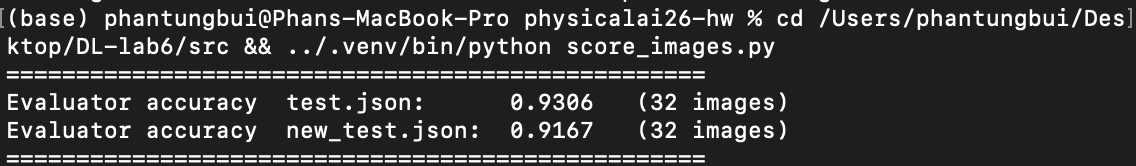
\includegraphics[width=0.85\linewidth]{figures/evaluator.png}}
\caption{Evaluator output for the submitted PNG files: 0.9306 on \texttt{test.json} and 0.9167 on \texttt{new\_test.json}. The script loads each saved image, applies the mean 0.5 / standard deviation 0.5 normalization, and calls the provided \texttt{eval}.}
\label{fig:screens}
\end{figure}

\subsection{Generated images}\label{sec:grids}
Figures~\ref{fig:grid_test} and~\ref{fig:grid_new} show all 32 generated images for each
test file, in list order, eight per row. Objects have the requested colors and shapes,
realistic shading and shadows, and plausible scene layouts.

Scoring each saved PNG individually reproduces the reported accuracies exactly, so
saving to 8-bit PNG loses nothing. The 12 missed objects (5 in 4 \texttt{test.json}
images, 7 in 6 \texttt{new\_test.json} images) all occur in three-object scenes:
\begin{itemize}
\item \textbf{Shape confusions} are the most common error (6 of the 10 failing images),
and all of them are between cubes and cylinders, for example a red cylinder generated
instead of a red cube. Both shapes have flat tops and vertical sides, and at
$64\times64$ they differ by only a few pixels of edge shading.
\item \textbf{Color confusions} occur between neighboring hues in two images: brown
generated as red, and blue as cyan. One further \texttt{test.json} image misses two
objects through a mix of color and shape errors.
\item \textbf{Attribute binding} fails once (two missed objects). For \{brown cube, purple cube, red cylinder\},
the image contains a red cube and a brown cylinder: the right colors and shapes, attached
to the wrong objects. Summing per-object label embeddings into one vector does not record
which color belongs to which shape, so this is a known weakness of the multi-hot
conditioning. The condition itself is unambiguous here, since each listed name fixes
both color and shape, but the network has to recover the binding from a sum.
\end{itemize}

\begin{figure}[H]
\centering
\includegraphics[width=0.92\linewidth]{../outputs/final/grid_test.png}
\caption{Generated images for \texttt{test.json} (accuracy 0.931).}
\label{fig:grid_test}
\end{figure}

\begin{figure}[H]
\centering
\includegraphics[width=0.92\linewidth]{../outputs/final/grid_new_test.png}
\caption{Generated images for \texttt{new\_test.json} (accuracy 0.917).}
\label{fig:grid_new}
\end{figure}

\subsection{Denoising process}
Figure~\ref{fig:denoise} shows ten evenly spaced states $\x_t$ of the reverse process for
the condition \{blue cube, yellow sphere, purple cylinder\}, from pure noise on the left
to the final image on the right. Coarse structure appears first. The blurry colored blobs
that mark the object positions are visible about two-thirds of the way through, while
shapes, edges, and shading are only resolved in the last steps. This matches the usual
view of diffusion as coarse-to-fine generation. The evaluator recognizes all three
requested objects in the final image.

\begin{figure}[H]
\centering
\includegraphics[width=\linewidth]{../outputs/final/denoising_process.png}
\caption{Denoising process for \{blue cube, yellow sphere, purple cylinder\}, ordered from noisy to clear.}
\label{fig:denoise}
\end{figure}

\subsection{Experiment 1: the first sampling timestep}\label{sec:tstart}
The first full run sampled from $t=999$ and scored only 0.694 and 0.786. Inspecting the
grids showed that many images were still covered in saturated per-pixel color noise,
while the others were clean, which pointed to a problem in the sampler rather than in
the conditioning.

The cause is the cosine schedule's last step. Clipping $\beta_{999}$ at 0.999 makes
$\abar_{999}\approx2.4\times10^{-9}$, so
$\hat{\x}_0=(\x_t-\sqrt{1-\abar_t}\hat{\eps})/\sqrt{\abar_t}$ multiplies any prediction
error by about 20,000. Clipping then turns that error into a saturated $\pm1$ pattern that
later steps do not fully remove. In the lecture's $\sigma$ parameterization, $t=999$ corresponds to
$\sigma\approx2\times10^{4}$, far beyond the typical $\sigma_\text{max}=100$, while
$t=960$ corresponds to $\sigma\approx16$.

Starting the DDIM trajectory slightly later fixes the problem without retraining
(Table~\ref{tab:tstart}, Figure~\ref{fig:sweeps} left). At these timesteps the signal
fraction $\sqrt{\abar_t}$ is still below 0.16, so starting from pure Gaussian noise
remains an accurate approximation. All start points from 980 to 900 score above 0.84 on
both files. I chose $t_1=960$ from the middle of this plateau rather than the single best
value, because each test file has only 32 images, and one misrecognized object changes
the accuracy by 0.014 on \texttt{test.json} (72 objects) and 0.012 on
\texttt{new\_test.json} (84 objects).

\begin{table}[H]
\centering\small
\begin{tabular}{rccccc}
\toprule
First timestep $t_1$ & 999 & 980 & 960 & 940 & 900 \\
$\abar_{t_1}$ & $2.4\times10^{-9}$ & $8.8\times10^{-4}$ & $3.7\times10^{-3}$ & $8.4\times10^{-3}$ & $2.4\times10^{-2}$ \\
Equivalent $\sigma$ & 20,300 & 33.8 & 16.4 & 10.8 & 6.4 \\
\midrule
\texttt{test.json} & 0.667 & 0.847 & \textbf{0.875} & 0.861 & 0.847 \\
\texttt{new\_test.json} & 0.786 & 0.893 & 0.893 & 0.893 & \textbf{0.917} \\
\bottomrule
\end{tabular}
\caption{Effect of the first sampling timestep (CFG $w=3$, 100 DDIM steps, seed 0).}
\label{tab:tstart}
\end{table}

\subsection{Experiment 2: classifier-free guidance scale}
With the start point fixed at 960, I swept the guidance scale (Table~\ref{tab:cfg},
Figure~\ref{fig:sweeps} right). The purely conditional model ($w=1$) already reaches about
0.80, and guidance adds over 0.1. Accuracy peaks at $w=4$ and falls at $w=5$. This matches
the usual trade-off of CFG: stronger guidance improves agreement with the condition, but
too much extrapolation away from the unconditional prediction pushes samples off the data
distribution and reduces diversity and realism~\cite{ho2022cfg}.

\begin{table}[H]
\centering\small
\begin{tabular}{rccccc}
\toprule
CFG scale $w$ & 1 & 2 & 3 & 4 & 5 \\
\midrule
\texttt{test.json} & 0.792 & 0.847 & 0.875 & \textbf{0.931} & 0.875 \\
\texttt{new\_test.json} & 0.810 & 0.869 & 0.893 & \textbf{0.917} & 0.905 \\
\bottomrule
\end{tabular}
\caption{Effect of the CFG scale ($t_1=960$, 100 DDIM steps, seed 0).}
\label{tab:cfg}
\end{table}

\begin{figure}[H]
\centering
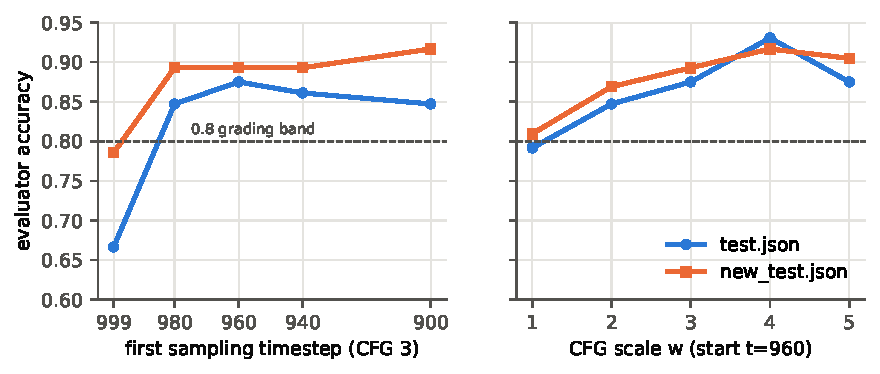
\includegraphics[width=\linewidth]{figures/sweeps.pdf}
\caption{Accuracy against the first sampling timestep (left) and the CFG scale (right). The dashed line marks 0.8, the top grading band.}
\label{fig:sweeps}
\end{figure}

\subsection{Experiment 3: classifier guidance}\label{sec:cg}
On top of CFG with $w=4$, I added classifier guidance with the frozen evaluator at three
weights (Table~\ref{tab:cg}). All three improve accuracy, and $s=1$ gives the best mean,
reaching 0.958 and 0.988. Very strong guidance ($s=10$) starts to hurt
\texttt{new\_test.json}.

\begin{table}[H]
\centering\small
\begin{tabular}{rcccc}
\toprule
Classifier-guidance weight $s$ & 0 (CFG only) & 1 & 3 & 10 \\
\midrule
\texttt{test.json} & 0.931 & 0.958 & 0.958 & \textbf{0.972} \\
\texttt{new\_test.json} & 0.917 & \textbf{0.988} & 0.976 & 0.929 \\
\bottomrule
\end{tabular}
\caption{Classifier guidance on top of CFG ($w=4$, $t_1=960$, 100 DDIM steps, seed 0).}
\label{tab:cg}
\end{table}

The guided images look natural, with the requested objects, normal shading, and no visible
adversarial patterns. However, the guiding classifier is the same network that computes the
score, so part of the gain may come from fitting that network's decision boundaries rather
than from better images, and the number overstates the improvement a human would see. For
this reason the submitted images use CFG only. Both settings are well inside the top
grading band.

\subsection{Experiment 4: robustness across random seeds}\label{sec:seeds}
All results above use seed 0. To check that they are not a lucky draw, I generated both
test sets again with seeds 1--3, with and without classifier guidance
(Table~\ref{tab:seeds}).

\begin{table}[H]
\centering\small
\begin{tabular}{llccccc}
\toprule
Setting & File & Seed 0 & Seed 1 & Seed 2 & Seed 3 & Mean $\pm$ s.d. \\
\midrule
CFG only & \texttt{test.json} & 0.931 & 0.931 & 0.903 & 0.917 & $0.920\pm0.013$ \\
 & \texttt{new\_test.json} & 0.917 & 0.881 & 0.893 & 0.964 & $0.914\pm0.037$ \\
\midrule
CFG + CG ($s=1$) & \texttt{test.json} & 0.958 & 0.958 & 0.958 & 0.972 & $0.962\pm0.007$ \\
 & \texttt{new\_test.json} & 0.988 & 0.976 & 1.000 & 0.964 & $0.982\pm0.015$ \\
\bottomrule
\end{tabular}
\caption{Accuracy over four seeds ($w=4$, $t_1=960$, 100 DDIM steps).}
\label{tab:seeds}
\end{table}

Every seed stays above 0.88, so the final model is in the top band regardless of the draw.
The submitted seed 0 is close to the mean on both files. Classifier guidance improves
every seed and also reduces the spread. The spread on \texttt{new\_test.json} is larger
because a few hard three-object conditions are solved by some draws and not others. The
start-timestep fix also does not remove residual noise for every starting point: one of
the 32 \texttt{test.json} images for seed 1 with classifier guidance still showed visible
noise, which suggests that starting even later
or training longer would help further.

\subsection{Experiment 5: training dynamics}
Figure~\ref{fig:train} shows the training loss and the accuracy measured during training.
The loss drops sharply in the first epochs and then decreases slowly. Its absolute value is
small because most of each i-CLEVR image is a flat gray background that is easy to denoise.
The accuracy during training was measured with the original sampler ($t_1=999$, $w=2$,
50 steps), so its absolute level is depressed by the residual-noise problem. Its trend is
still informative: accuracy rises quickly for about 30 epochs and then improves slowly, and
it had not clearly saturated when the time budget ended at epoch 123. Longer training would
likely help further, but the corrected sampler already reaches the top grading band with
this checkpoint.

\begin{figure}[H]
\centering
\begin{subfigure}{0.48\linewidth}\centering
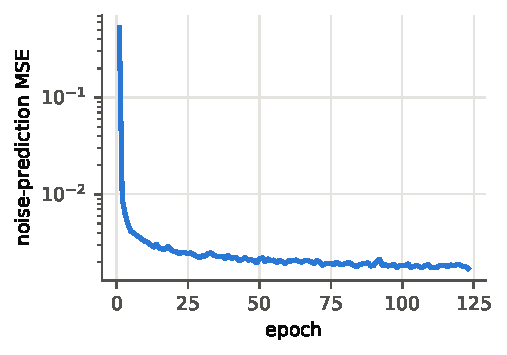
\includegraphics[width=\linewidth]{figures/loss.pdf}
\caption{Training loss (log scale).}
\end{subfigure}\hfill
\begin{subfigure}{0.48\linewidth}\centering
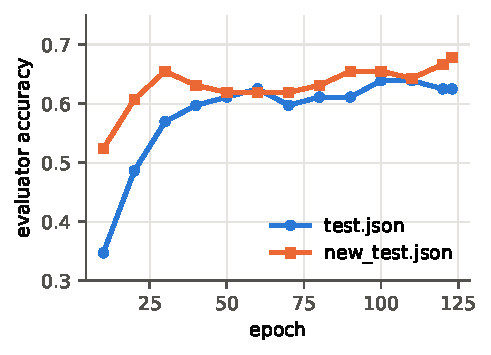
\includegraphics[width=\linewidth]{figures/train_acc.pdf}
\caption{Accuracy during training (sampler with $t_1=999$).}
\end{subfigure}
\caption{Training dynamics over 123 epochs.}
\label{fig:train}
\end{figure}

\subsection{Discussion}
\begin{itemize}
\item \textbf{The sampler mattered more than extra training.} With everything else fixed,
changing only the first sampling timestep from 999 to 960 raised accuracy by about 0.21
on \texttt{test.json} (Table~\ref{tab:tstart}), far more than the last 90 epochs of
training did.
\item \textbf{CFG is the main conditioning lever.} One network trained with 10\% label
dropout supports any guidance scale at test time, and tuning $w$ alone added more than 0.1.
\item \textbf{Limitations.} Each test file has only 32 conditions, so differences of one or
two objects are within noise (Section~\ref{sec:seeds} quantifies the seed-to-seed
variation). The lab provides no separate validation conditions, so the start timestep
and guidance scale were selected on the test conditions themselves. Both are sampler
settings rather than trained parameters, and the plateaus in Figure~\ref{fig:sweeps} are
wide, but the reported accuracies are still slightly optimistic. Training stopped because
of the time budget, not convergence.
\end{itemize}

%=====================================================================
\begin{thebibliography}{9}\small
\bibitem{ho2020} J.~Ho, A.~Jain, P.~Abbeel. Denoising Diffusion Probabilistic Models. \emph{NeurIPS}, 2020.
\bibitem{nichol2021} A.~Nichol, P.~Dhariwal. Improved Denoising Diffusion Probabilistic Models. \emph{ICML}, 2021.
\bibitem{song2021ddim} J.~Song, C.~Meng, S.~Ermon. Denoising Diffusion Implicit Models. \emph{ICLR}, 2021.
\bibitem{ho2022cfg} J.~Ho, T.~Salimans. Classifier-Free Diffusion Guidance. \emph{NeurIPS Workshop}, 2021. arXiv:2207.12598.
\bibitem{dhariwal2021} P.~Dhariwal, A.~Nichol. Diffusion Models Beat GANs on Image Synthesis. \emph{NeurIPS}, 2021.
\end{thebibliography}

\end{document}
